\section{Kameramodell} \label{sec:kameramodell}
Da das verwendete Fisheye-Objektiv durch seinen großen Blickwinkel stark verzerrt auf den Kamerasensor abbildet, ist ein spezielles Kameramodell zur Rektifizierung der Bilddaten notwendig. Wir haben uns in dieser Arbeit für die Nutzung einer Matlab-Toolbox entschieden  \autocite{OCamCalibOmnidirectionalCamera, scaramuzzaFlexibleTechniqueAccurate2006, scaramuzzaToolboxEasilyCalibrating2006, scaramuzzaOmnidirectionalVisionCalibration2007, rufliAutomaticDetectionCheckerboards2008}. Das in selbiger verwendete Modell und die Anwendung dessen zur Entzerrung soll nun erläutert werden. 

Die OcamCalib-Toolbox behandelt das Kamerasystem als Einheit, d.h. die Kamera und der Fisheyeobjektivaufsatz (alternativ der konvexe Spiegel) werden zusammen durch einen Parametersatz beschrieben.

Das Modell hat das Ziel, den Zusammenhang zwischen einem Punkt auf dem Bildsensor \gls{lat:camerapoint} mit Koordinaten (u,v) und einem vom optischen Zentrum des Objektivs ausgehenden Vektors nicht festgelegter Länge \gls{lat:cameravector} mit Koordinaten (x,y,z) zu finden (s.~\eqref{eq:ocamcalibuv}).

\begin{figure}[H]
  \centering
  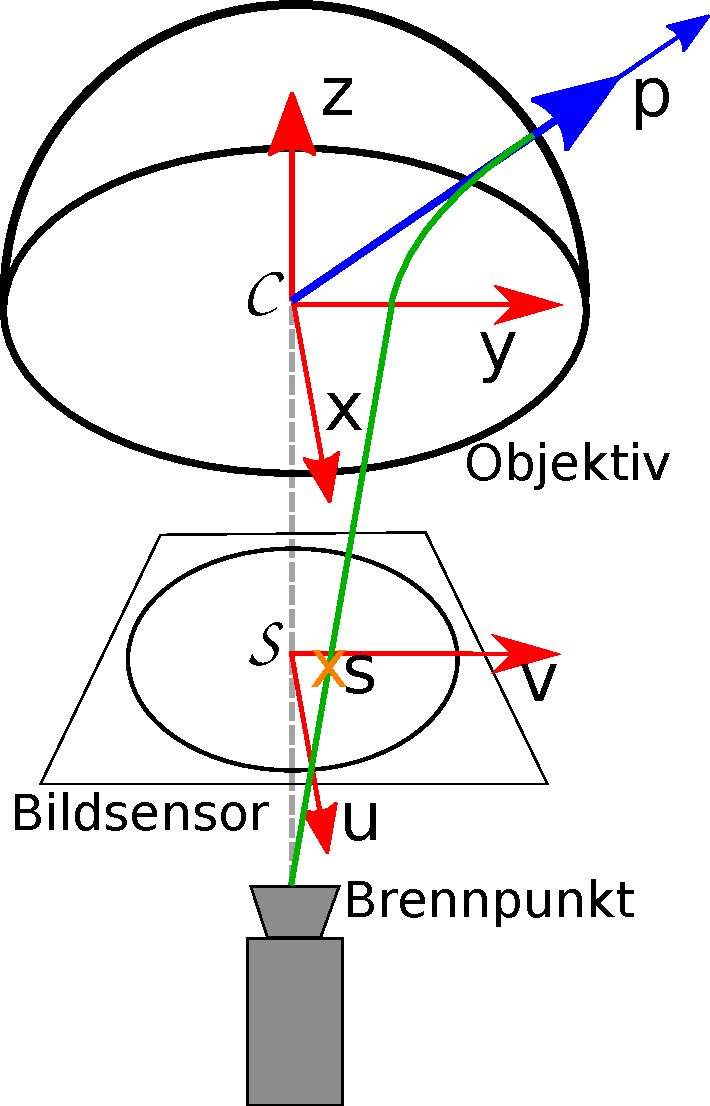
\includegraphics[width=0.5\textwidth]{OCamCalib_Kameramodell}
  \caption{Das Kameramodell der OCamCalib Toolbox}
  \label{fig:kameramodell}
\end{figure}

\subsection{Annahmen}
Im verwendeten Modell werden folgende Annahmen getroffen:
\begin{enumerate}
\item Die verwendete Optik stellt ein zentrales Kamerasystem dar, d.h. alle einfallenden Strahlen, welche sich im Brennpunkt des Objektivs nach der Brechung schneiden (s. grüner Strahlverlauf in~\ref{fig:kameramodell}), schneiden sich auch ungebrochen in einem Punkt (s. blauer Strahlverlaufin~\ref{fig:kameramodell}). Dieser Punkt ist das optische Zentrum des Objektivs und der Koordinatenursprung des Kamerakoordinatensystems \gls{lat:OCKOS}.
\item \label{item:ocamcalibassm2} Die Achse des Bildsensors und des Objektivs sind nahezu identisch (s. unterbrochene graue Linie in~\ref{fig:kameramodell}). Das Modell berücksichtigt nur kleine Abweichungen der Rotationen der Achsen gegeneinander.
\item Das Objektiv ist rotationssymetrisch zu seiner Achse(s. unterbrochene graue Linie in~\ref{fig:kameramodell}).
\item Die Linsenverzerrung wird nicht durch herkömmliche Methoden, sondern durch die Projektionsfunktion \fnf{\gls{x}_{\gls{lat:OSKOS}},\gls{y}_{\gls{lat:OSKOS}}}~\eqref{eq:ocamcalibuv} berücksichtigt.
\end{enumerate}

\subsection{Herleitung}
Da die Objektivachse und die Achse des Bildsensors in erster Näherung gleich sind, lässt sich schreiben:
\begin{equation}
\begin{pmatrix}
\gls{x}_{\gls{lat:OCKOS}} \\ \gls{y}_{\gls{lat:OCKOS}}
\end{pmatrix}
= \gls{gre:repos} \cdot
\begin{pmatrix}
\gls{x}_{\gls{lat:OSKOS}} \\ \gls{y}_{\gls{lat:OSKOS}}
\end{pmatrix}
\end{equation}
Der gesuchte Zusammenhang lautet: 
\begin{equation}
\gls{lat:cameravector} =
\begin{pmatrix}
\gls{x}_{\gls{lat:OCKOS}} \\ \gls{y}_{\gls{lat:OCKOS}} \\ \gls{z}_{\gls{lat:OCKOS}}
\end{pmatrix}
=
\begin{pmatrix}
\gls{gre:repos} \cdot \gls{x}_{\gls{lat:OSKOS}} \\  \gls{gre:repos} \cdot \gls{y}_{\gls{lat:OSKOS}} \\ \fnf{\gls{x}_{\gls{lat:OSKOS}},\gls{y}_{\gls{lat:OSKOS}}}
\end{pmatrix}
\end{equation}
Der Faktor  \gls{gre:repos} kann in die Funktion \fnf{\gls{x}_{\gls{lat:OSKOS}},\gls{y}_{\gls{lat:OSKOS}}} integriert werden:
\begin{equation}
\label{eq:ocamcalibuv}
\gls{lat:cameravector} =
\begin{pmatrix}
\gls{x}_{\gls{lat:OCKOS}} \\ \gls{y}_{\gls{lat:OCKOS}} \\ \gls{z}_{\gls{lat:OCKOS}}
\end{pmatrix}
=
\begin{pmatrix}
\gls{x}_{\gls{lat:OSKOS}} \\ \gls{y}_{\gls{lat:OSKOS}} \\ \fnf{\gls{x}_{\gls{lat:OSKOS}},\gls{y}_{\gls{lat:OSKOS}}}
\end{pmatrix}
\end{equation}
Da da das Objektiv rotationssymetrisch ist, kann \fnf{\gls{x}_{\gls{lat:OSKOS}},\gls{y}_{\gls{lat:OSKOS}}} nur vom Abstand eines Punktes vom Mittelpunkt des Bildsensors abhängig gemacht werden:
\begin{equation}
\label{eq:ocamcalibdist}
\gls{gre:distsensorcenter}=\sqrt{\gls{x}_{\gls{lat:OSKOS}}^2+\gls{y}_{\gls{lat:OSKOS}}^2}
\end{equation}
Aus~\eqref{eq:ocamcalibuv}~und~\eqref{eq:ocamcalibdist} ergibt sich: 
\begin{equation}
\label{eq:ocamcalibfin}
\gls{lat:cameravector} =
\begin{pmatrix}
\gls{x}_{\gls{lat:OCKOS}} \\ \gls{y}_{\gls{lat:OCKOS}} \\ \gls{z}_{\gls{lat:OCKOS}}
\end{pmatrix}
=
\begin{pmatrix}
\gls{x}_{\gls{lat:OSKOS}} \\ \gls{y}_{\gls{lat:OSKOS}} \\ \fnf{(\gls{gre:distsensorcenter})}
\end{pmatrix}
\end{equation}
Die Aufgabe der Kalibration besteht nun im Ermitteln der Funktion \fnf{(\gls{gre:distsensorcenter})}~\eqref{eq:ocamcalibrho}, welche in der Toolbox durch ein Polynom 4. Grades approximiert wird:
\begin{equation}
\label{eq:ocamcalibrho}
 f(\rho) = a_0 + a_1 \rho + a_2 \rho^2 + a_3 \rho^3 + a_4 \rho^4
\end{equation}
Da ein Darlegen des Prozesses zur Ermittlung der Parameter \(a_0 \dots a_4 \)  den Rahmen dieser Arbeit sprengen würde, wird darauf verzichtet.

\subsection{Entzerrung}

\begin{figure}[H]
  \centering
  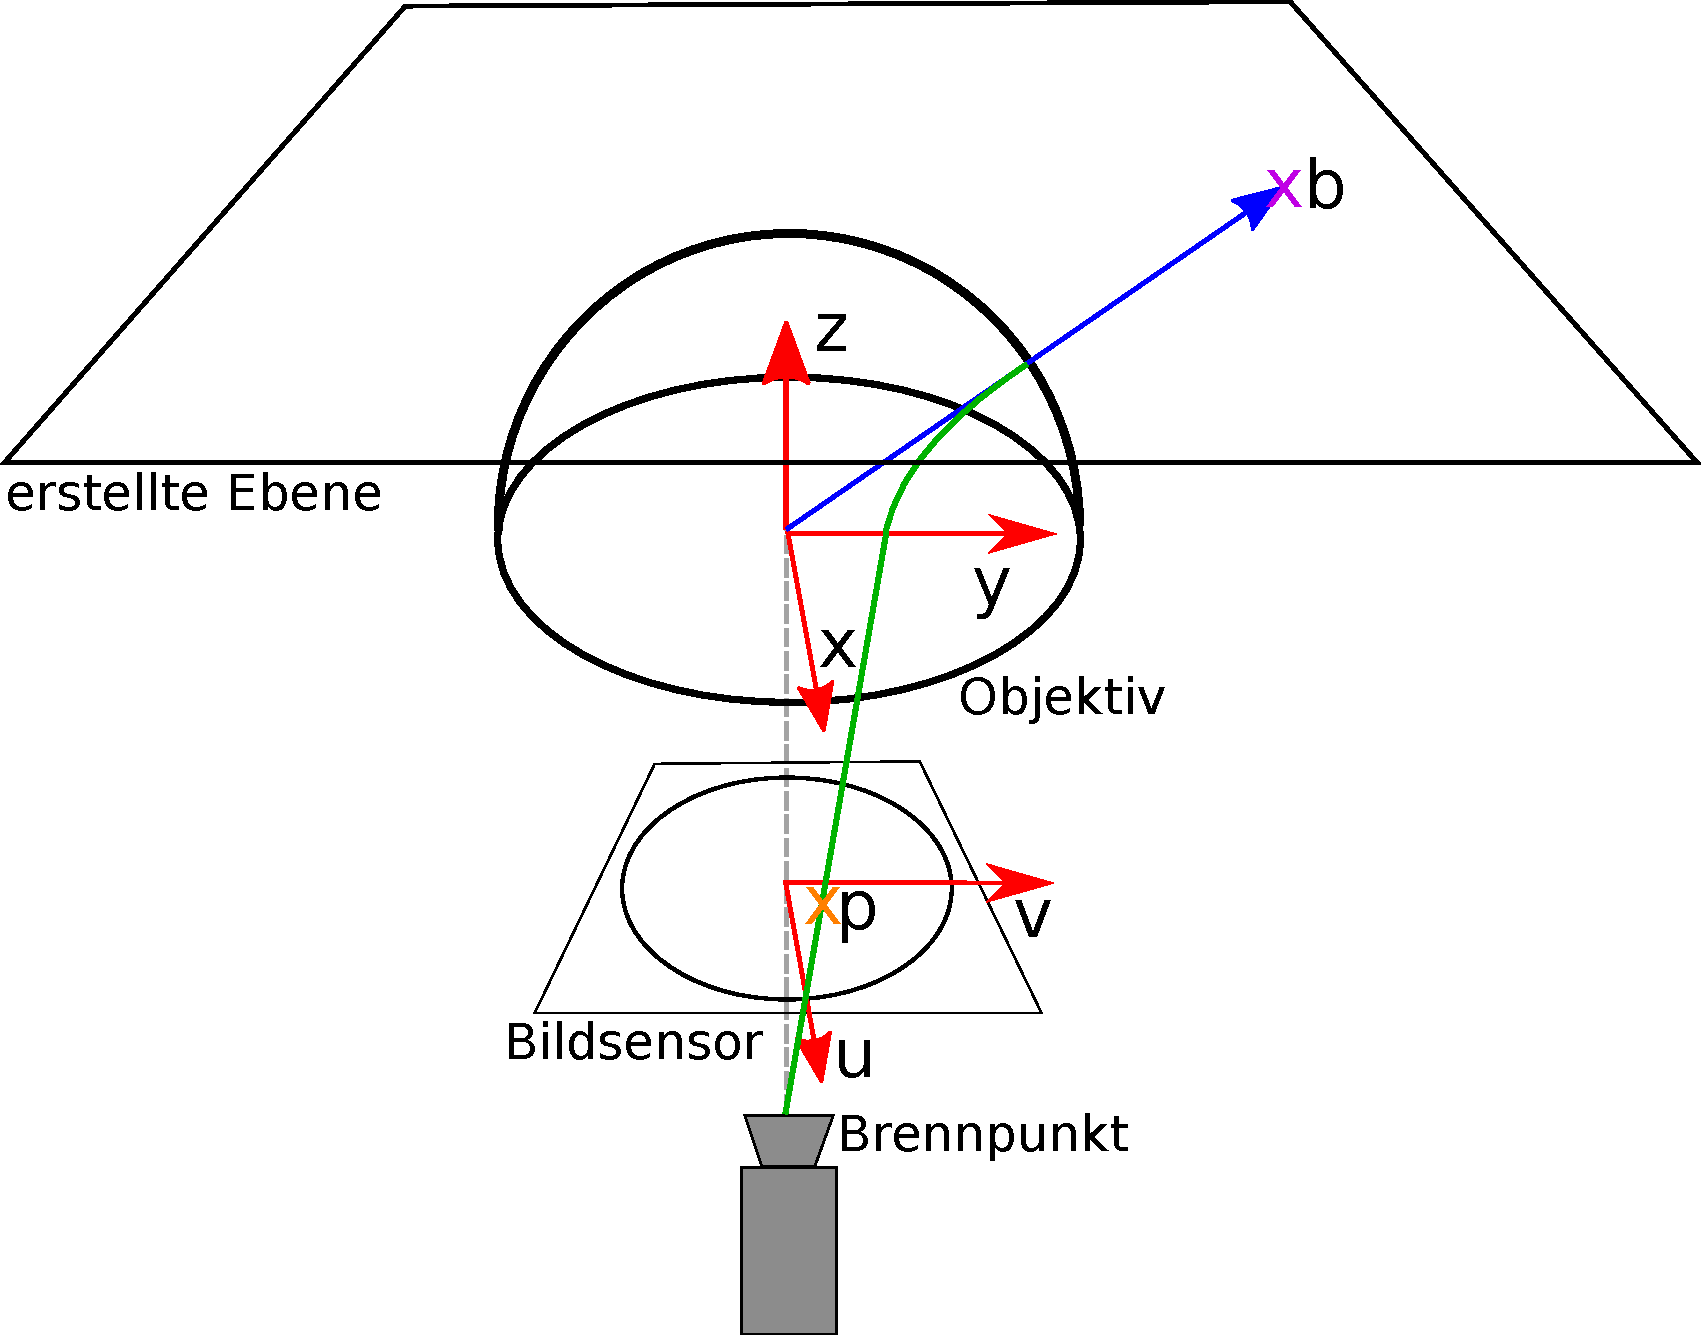
\includegraphics[width=0.75\textwidth]{OCamCalib_Kameramodell_Ebene}
  \caption{Entzerrung mit dem Kameramodell der OCamCalib Toolbox}
  \label{fig:kameramodell_entzerrung}
\end{figure}

Mithilfe der gewonnenen Informationen kann die Entzerrung des Bildes nun stattfinden. Zuerst wird eine Ebene parallel zur xy-Ebene des Kamerakoordinatensystems xyz erstellt. Die z-Koordinate ist hierbei wählbar. Diese Ebene wird nun in eine Menge von Punkten diskretisiert. Im entstandenen zweidimensionalen Array kann jedem Element ein Vektor (x,y,z) zugeordnet werden  (z.B. Punkt b in \ref{fig:kameramodell_entzerrung}). Durch Gleichung~\eqref{eq:ocamcalibfin} lassen sich diesem Vektor Koordinaten (u,v) auf dem Kamerasensor zuordnen. Das Pixel mit dem geringsten Abstand zu den gewünschten Koordinaten (u,v) liefert nun den Farbwert für jeden Punkt der Ebene, welche das entzerrte Bild darstellt.

\subsection{Affine Transformation}
Da Annahme~\ref{item:ocamcalibassm2} in der Realität nie exakt zutrifft  und bei der Digitalisierung des Bildes durch den Kamerasensor mit nichtquadratischen Pixeln zu rechnen ist, muss vor der Nutzung des hergeleiteten Modells eine affine Transformation der realen Koordinaten (u',v') in die idealen Koorinaten (u,v) stattfinden.
\begin{equation}
\begin{pmatrix}
u' \\ v' 
\end{pmatrix}
=
\begin{pmatrix}
 c & d \\
 e & 1 
\end{pmatrix}
\cdot
\begin{pmatrix}
u \\ v 
\end{pmatrix}
+
\begin{pmatrix}
xc' \\ yc' 
\end{pmatrix}
\end{equation}
 Die Verschiebung des Bildmittelpunktes (xc',yc') sowie die Parameter c,d,e werden im Kalibrationsprozess durch die Toolbox ermittelt.


